%%
%% $Id$
%%
%% Copyright (c) 2007-2009 Christian Fehler
%% Copyright (c) 2007-2009 Benjamin Mies
%%


\chapter{Sonstiges}


\section{Algorithmen}

In allen Algorithmen-Fenstern gibt es einen Button "`Algorithmus anzeigen"'. Dann erscheint ein Fenster ähnlich dem Folgenden.

\begin{figure}[h]
\begin{center}
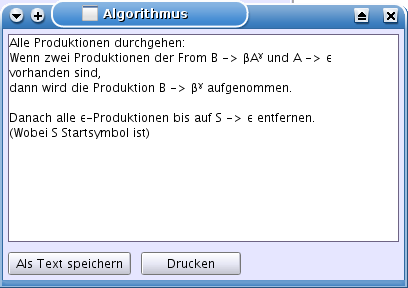
\includegraphics[width=6cm]{../images/algorithms.png}
\caption{Algorithmenfenster}
\end{center}
\end{figure}

In diesem Fenster kann man sich den Algorithmus, welcher gerade ausgeführt wird in Kurzform noch einmal anschauen. Während das Fenster geöffnet ist kann man trotzdem den Algorithmus laufen lassen. Es bleibt dann im Vordergrund.

Diesen Text kann man entweder als Textdatei speichern oder drucken.



\section{Zweite Ansicht}

Im Menüpunkt "`Ansicht"' ist die Option "`Zweite Ansicht"' zu finden. Wird dieser
Menüeintrag ausgewählt, wird eine zweite Ansicht eingeblendet, in der Dateien
geöffnet werden können. Dabei ist darauf zu achten, dass keine Dateien geöffnet
werden können, die bereits in der anderen Ansicht geöffnet sind. Wird trotzdem
eine solche Datei geöffnet, wird die Datei ausgewählt. Da immer nur eine Datei
aktiv sein kann, wird die aktive Ansicht durch eine dunklere Umrandung
dargestellt, als das bei der nicht aktiven der Fall ist. Die Button Stati
beziehen sich dann auf diese aktive Ansicht. Die aktive Ansicht kann durch
einfaches Anklicken einer Komponente in der Ansicht geändert werden.\vspace{10pt}

\begin{figure}[h]
\begin{center}
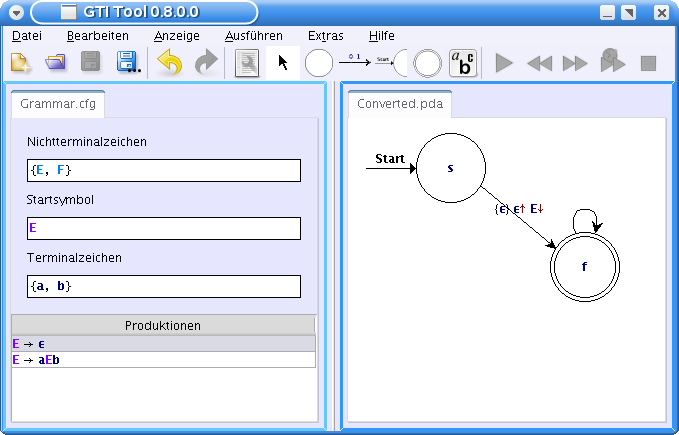
\includegraphics[width=12cm]{../images/second_view.png}
\caption{Zweite Ansicht}
\end{center}
\end{figure}

Um die Dateien in der anderen Ansicht zu öffnen, gibt es zwei verschiedene
Möglichkeiten. Zum einen kann die zweite Ansicht durch Anklicken aktiviert,
anschließend eine neue Datei erstellt oder eine bestehende geöffnet werden.
Eine andere Möglichkeit ist das Verschieben von geöffneten Dateien. Dies ist
möglich, indem auf einem Tab das Popupmenü geöffnet wird. Über "`Nach rechts
verschieben"' oder "`Nach links verschieben"' können die Dateien in die andere
Ansicht verschoben werden. Eine zweite Möglichkeit ist, das ebenfalls auch für
das normale Umsortieren von Tabs verfügbare, Verschieben per Drag and Drop.
Dazu kann ein Tab einfach in die andere Ansicht gezogen und dort an der richtigen
Stelle wieder losgelassen werden.\vspace{10pt}

Wird die zweite Ansicht wieder geschlossen, werden alle
geöffneten Dateien auf die normale Ansicht verschoben. Beim Verlassen des
Programmes wird gespeichert, welche Dateien auf welcher Ansicht geöffnet waren.


\section{Austausch von Dateien}

Das \gtitool bietet die Möglichkeit, geöffnete Dateien zu versenden und Dateien
von anderen \gtitool Benutzern zu empfangen. Zu erreichen ist der Austausch über
den Hauptmenüeintrag "`Extras"'. Die Dateien werden verschlüsselt
übertragen.\vspace{10pt}

Wenn eine Datei verschickt werden soll, muss diese als erstes selektiert werden.
Anschließend muss der Austausch Dialog geöffnet werden. Dieser bietet die
Möglichkeit, zwischen "`Senden"' und "`Empfangen"' zu wählen. Um die Datei zu
verschicken, muss also "`Senden"' ausgewählt werden, außerdem muss der "`Host"'
angegeben werden, auf dem ein \gtitool empfangsbereit ist. Zusätzlich ist der
"`Port"' anzugeben, standardmäßig ist Port "`64528"' eingestellt. Der Port muss
also nur geändert werden, wenn der Empfänger der Datei ihn ebenfalls geändert
hat. Beim Senden kann zusätzlich ein Kommentar vergeben werden, den der Empfänger
angezeigt bekommt, wenn die Datei empfangen wurde, der aber sonst keinen
Einfluss hat. Wenn alle Werte eingestellt sind, kann die Datei mit
"`Ausführen"' verschickt werden.\vspace{10pt}

\begin{figure}[h]
\begin{center}
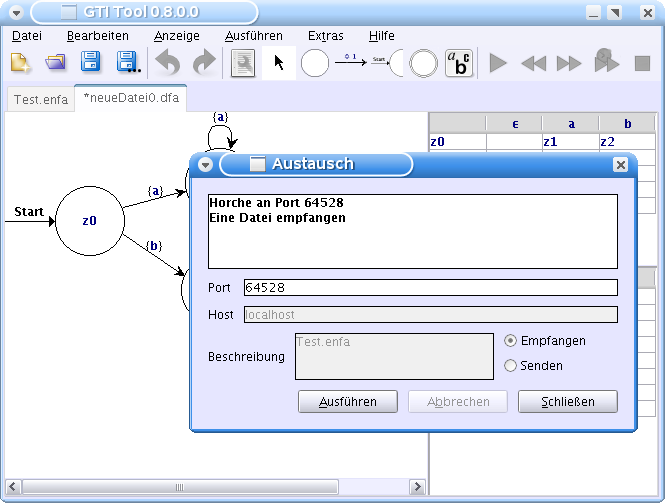
\includegraphics[width=12cm]{../images/exchange.png}
\caption{Austausch von Dateien}
\end{center}
\end{figure}

Das Empfangen einer Datei funktioniert sehr einfach, es muss nur der Port
eingestellt werden, auf dem der Server auf eingehende Dateien horchen soll. Per
"`Ausführen"' horcht der Server auf dem eingestellten Port auf eintreffende
Dateien. Per "`Abbrechen"' kann der Server wieder gestoppt werden, sollte keine
Datei empfangen werden. Wird eine Datei empfangen, wird diese automatisch
geöffnet und der Server beendet. Der Austausch Dialog wird nicht geschlossen, so
dass weitere Dateien empfangen oder verschickt werden können. Wird eine Datei
empfangen, kann der vom Sender eingestellte Kommentar im Nachrichtenfenster
eingesehen werden.


\section{Bild exportieren}

Im Menüpunkt "`Datei"' besteht die Möglichkeit, den Automaten Graphen in ein
Bild zu exportieren. Der Eintrag ist nur aktiv, wenn eine Automaten Datei
selektiert ist. Wird der Eintrag "`Bild exportieren"' angeklickt, öffnet sich
ein Speichern Dialog, mit dem das Bild gespeichert werden kann. Damit das
Ergebnis nicht zu viele freie Bereiche enthält, wird nur der vom Automaten
benutzte Bereich exportiert, zusätzlich zu einem 20 Pixel breiten Rand.
